\documentclass[12]{amsbook}

\usepackage{amssymb,amsmath}

%\usepackage{refcheck}

\usepackage{graphicx}
\usepackage{amssymb}
\usepackage{mathrsfs}
\usepackage{amsmath}
\usepackage{latexsym}
\usepackage{amssymb}
\usepackage{enumerate}
\usepackage{fullpage} 
\usepackage{setspace}
\usepackage{color}
%\usepackage{ dsfont }
\usepackage{float}
\usepackage{physics}
\usepackage{hyperref}

%new math symbols taking no arguments
\newcommand\0{\mathbf{0}}
\newcommand\CC{\mathbb{C}}
\newcommand\FF{\mathbb{F}}
\newcommand\NN{\mathbb{N}}
\newcommand\QQ{\mathbb{Q}}
\newcommand\RR{\mathbb{R}}
\newcommand\ZZ{\mathbb{Z}}
\newcommand\bb{\mathbf{b}}
\newcommand\kk{\Bbbk}
\newcommand\mm{\mathfrak{m}}
\newcommand\pp{\mathfrak{p}}
\newcommand\xx{\mathbf{x}}
\newcommand\yy{\mathbf{y}}
\newcommand\GL{\mathit{GL}}
\newcommand\into{\hookrightarrow}
\newcommand\nsub{\trianglelefteq}
\newcommand\onto{\twoheadrightarrow}
\newcommand\minus{\smallsetminus}
\newcommand\goesto{\rightsquigarrow}
\newcommand\nsubneq{\vartriangleleft}

%redefined math symbols taking no arguments
\newcommand\<{\langle}
\renewcommand\>{\rangle}
\renewcommand\iff{\Leftrightarrow}
\renewcommand\phi{\varphi}
\renewcommand\implies{\Rightarrow}

%new math symbols taking arguments
\newcommand\ol[1]{{\overline{#1}}}

%redefined math symbols taking arguments
\renewcommand\mod[1]{\ (\mathrm{mod}\ #1)}

%roman font math operators
\DeclareMathOperator\aut{Aut}

%for easy 2 x 2 matrices
\newcommand\twobytwo[1]{\left[\begin{array}{@{}cc@{}}#1\end{array}\right]}

%for easy column vectors of size 2
\newcommand\tworow[1]{\left[\begin{array}{@{}c@{}}#1\end{array}\right]}

\newtheorem{theorem}{Theorem}[section]
\newtheorem{corollary}{Corollary}[theorem]
\newtheorem{lemma}[theorem]{Lemma}
\newtheorem{exercise}[theorem]{Exercise}
\newtheorem{definition}[theorem]{Definition}

\title{PHY 365L Final Project: Neural Circuits}
\author{Faris Sbahi}


\begin{document}
\maketitle

\begin{abstract}
In this project, we construct and study circuits which are meant to model the actions potentials of several classes of neurons. We aim to understand the fundamentals of electronics in addition to those of cell and molecular biology of nerve cells.
\end{abstract}

\chapter*{Introduction}

The essence of nervous system function is signaling, or transferring information. Signaling is essential for an organism to (1) sense information about its enviornment, (2) import this information into its brain where it can be processed, and (3) generate a behavioral response.

\chapter{Axons}

\section{Introduction}


\section{Circuit 1: A Pulse Type Neuron}
 
 We begin by considering a circuit with the following structure
 
\begin{figure}[H]
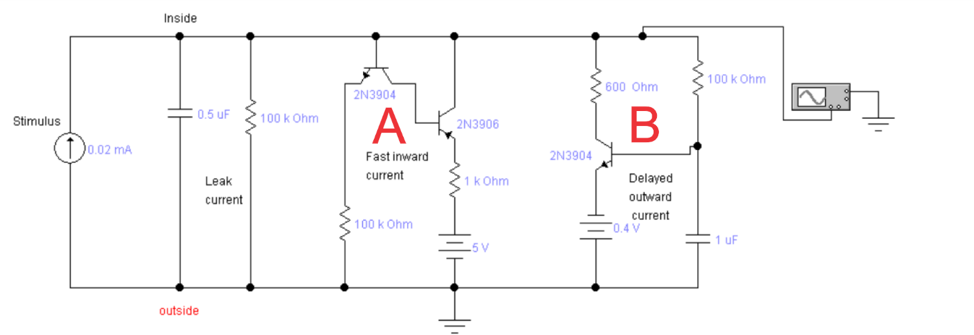
\includegraphics[width=0.5\textwidth]{exercise1-0}
\end{figure}

In our experiment, instead of applying a constant current source we added a $200k\Omega$ resistor above the $5V$ voltage source. Nevertheless, the analysis follows similarly.

Hence, we consider transistor sub-circuits A and B as ideal switches. When we just turn on the current source, the upper node voltage is equal to 0. Both switches are off, and the circuit could be reduced to the following circuit
 
 \begin{figure}[H]
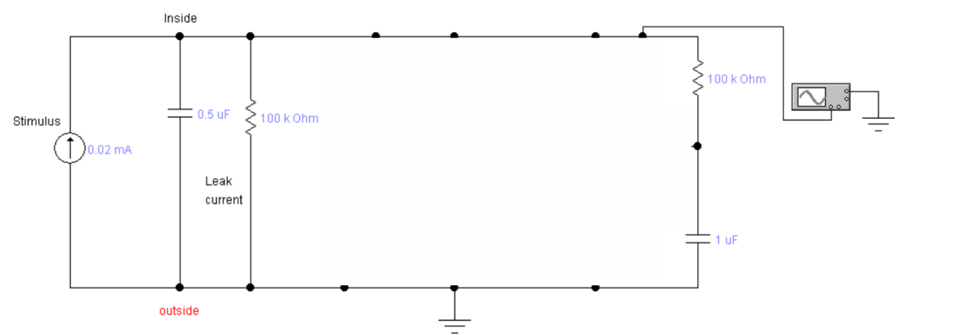
\includegraphics[width=0.5\textwidth]{exercise1-1}
\end{figure}

The dynamic of the upper node V(t) depends on the values of capacitors and resistors, but the final (equilibrium) voltage depends only on the stimulus current I and leak current resistor. If we are not interested in dynamics of V(t), but only in it’s equilibrium value, we can remove capacitors from the circuit.
 
 \begin{figure}[H]
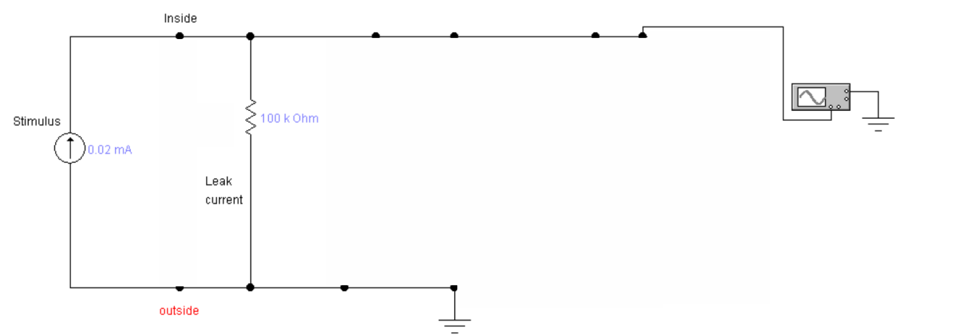
\includegraphics[width=0.5\textwidth]{exercise1-2}
\end{figure}

Clearly, this gives a voltage of $2V$ for the top node.

Now let’s turn on switch A
 
 \begin{figure}[H]
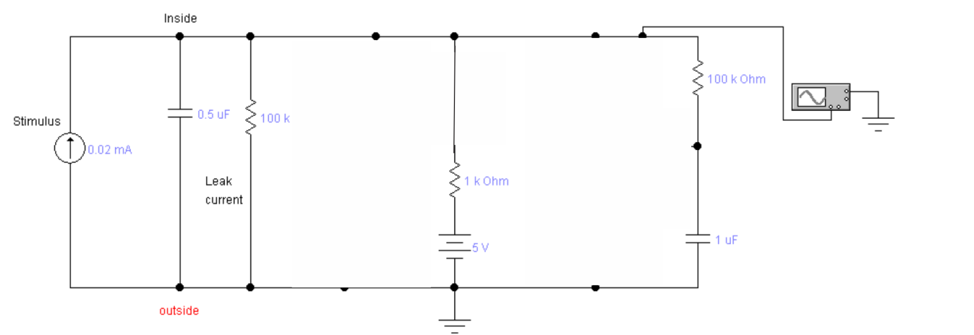
\includegraphics[width=0.5\textwidth]{exercise1-3}
\end{figure}

If we again are not interested in dynamics of V(t), we can redraw the circuit dropping all capacitors
 
 \begin{figure}[H]
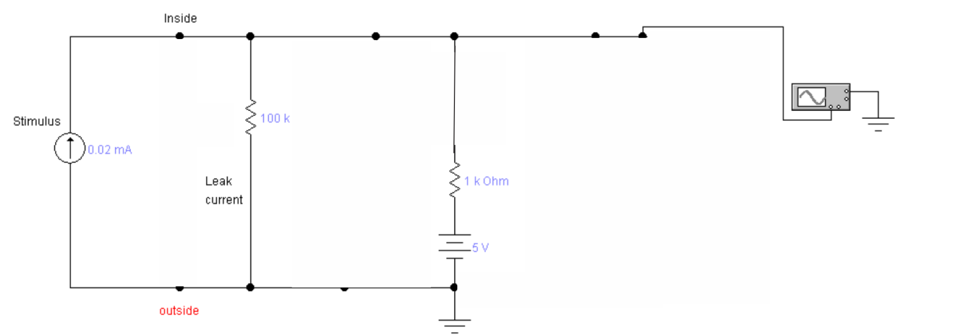
\includegraphics[width=0.5\textwidth]{exercise1-4}
\end{figure}

Find the voltage at the top node for this circuit.
And finally let’s turn on the switch B
 
 \begin{figure}[H]
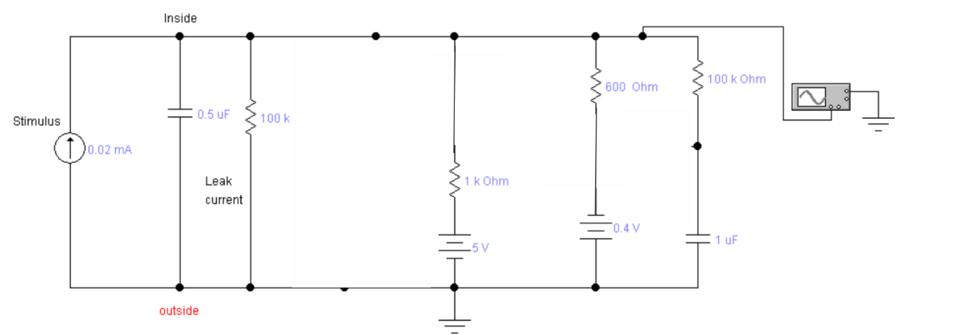
\includegraphics[width=0.5\textwidth]{exercise1-5}
\end{figure}

and drop all capacitors again
 
\begin{figure}[H]
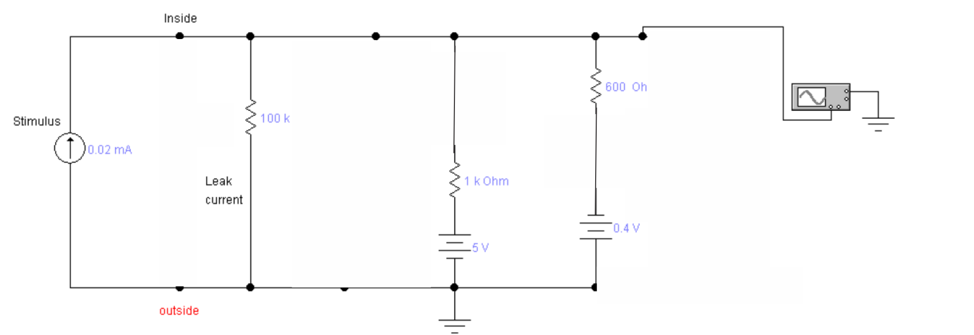
\includegraphics[width=0.5\textwidth]{exercise1-6}
\end{figure}

Find the voltage at the top node for this circuit.


\section{Circuit 2: A Pulse Type Neuron with Burst}

We've discussed that action potentials are fundamental to a neuron's ability to transfer information. However, there are additional aspects of its electrical properties which shape neuronal input and output. For example, some neurons that fire spontaneously in the absence of external simulation do not fire at regular intervals, but instead generate bursts of action potentials that are separated by the hyperpolarizations of the membrane. Such cells are terms "bursting" neurons \cite{levitan2015neuron}.

These bursts are used in at least two known ways \cite{levitan2015neuron}:

\begin{enumerate}
\item To generate rhythmic behaviors. For example, breathing, walking, swimming, and chewing food.	
\item To secrete neurohormones. For example, neurons located in the hypothalamic region of the mammalian brain individually contain either vasopressin or oxyocin. These hormones control water retention and lactation, respectively. Interestingly, it appears that the bursting pattern is more effective than a steady pacing pattern of firing as a stimulus to the intracellular mechanism which generates peptide release.
\end{enumerate}
 

\begin{figure}[H]
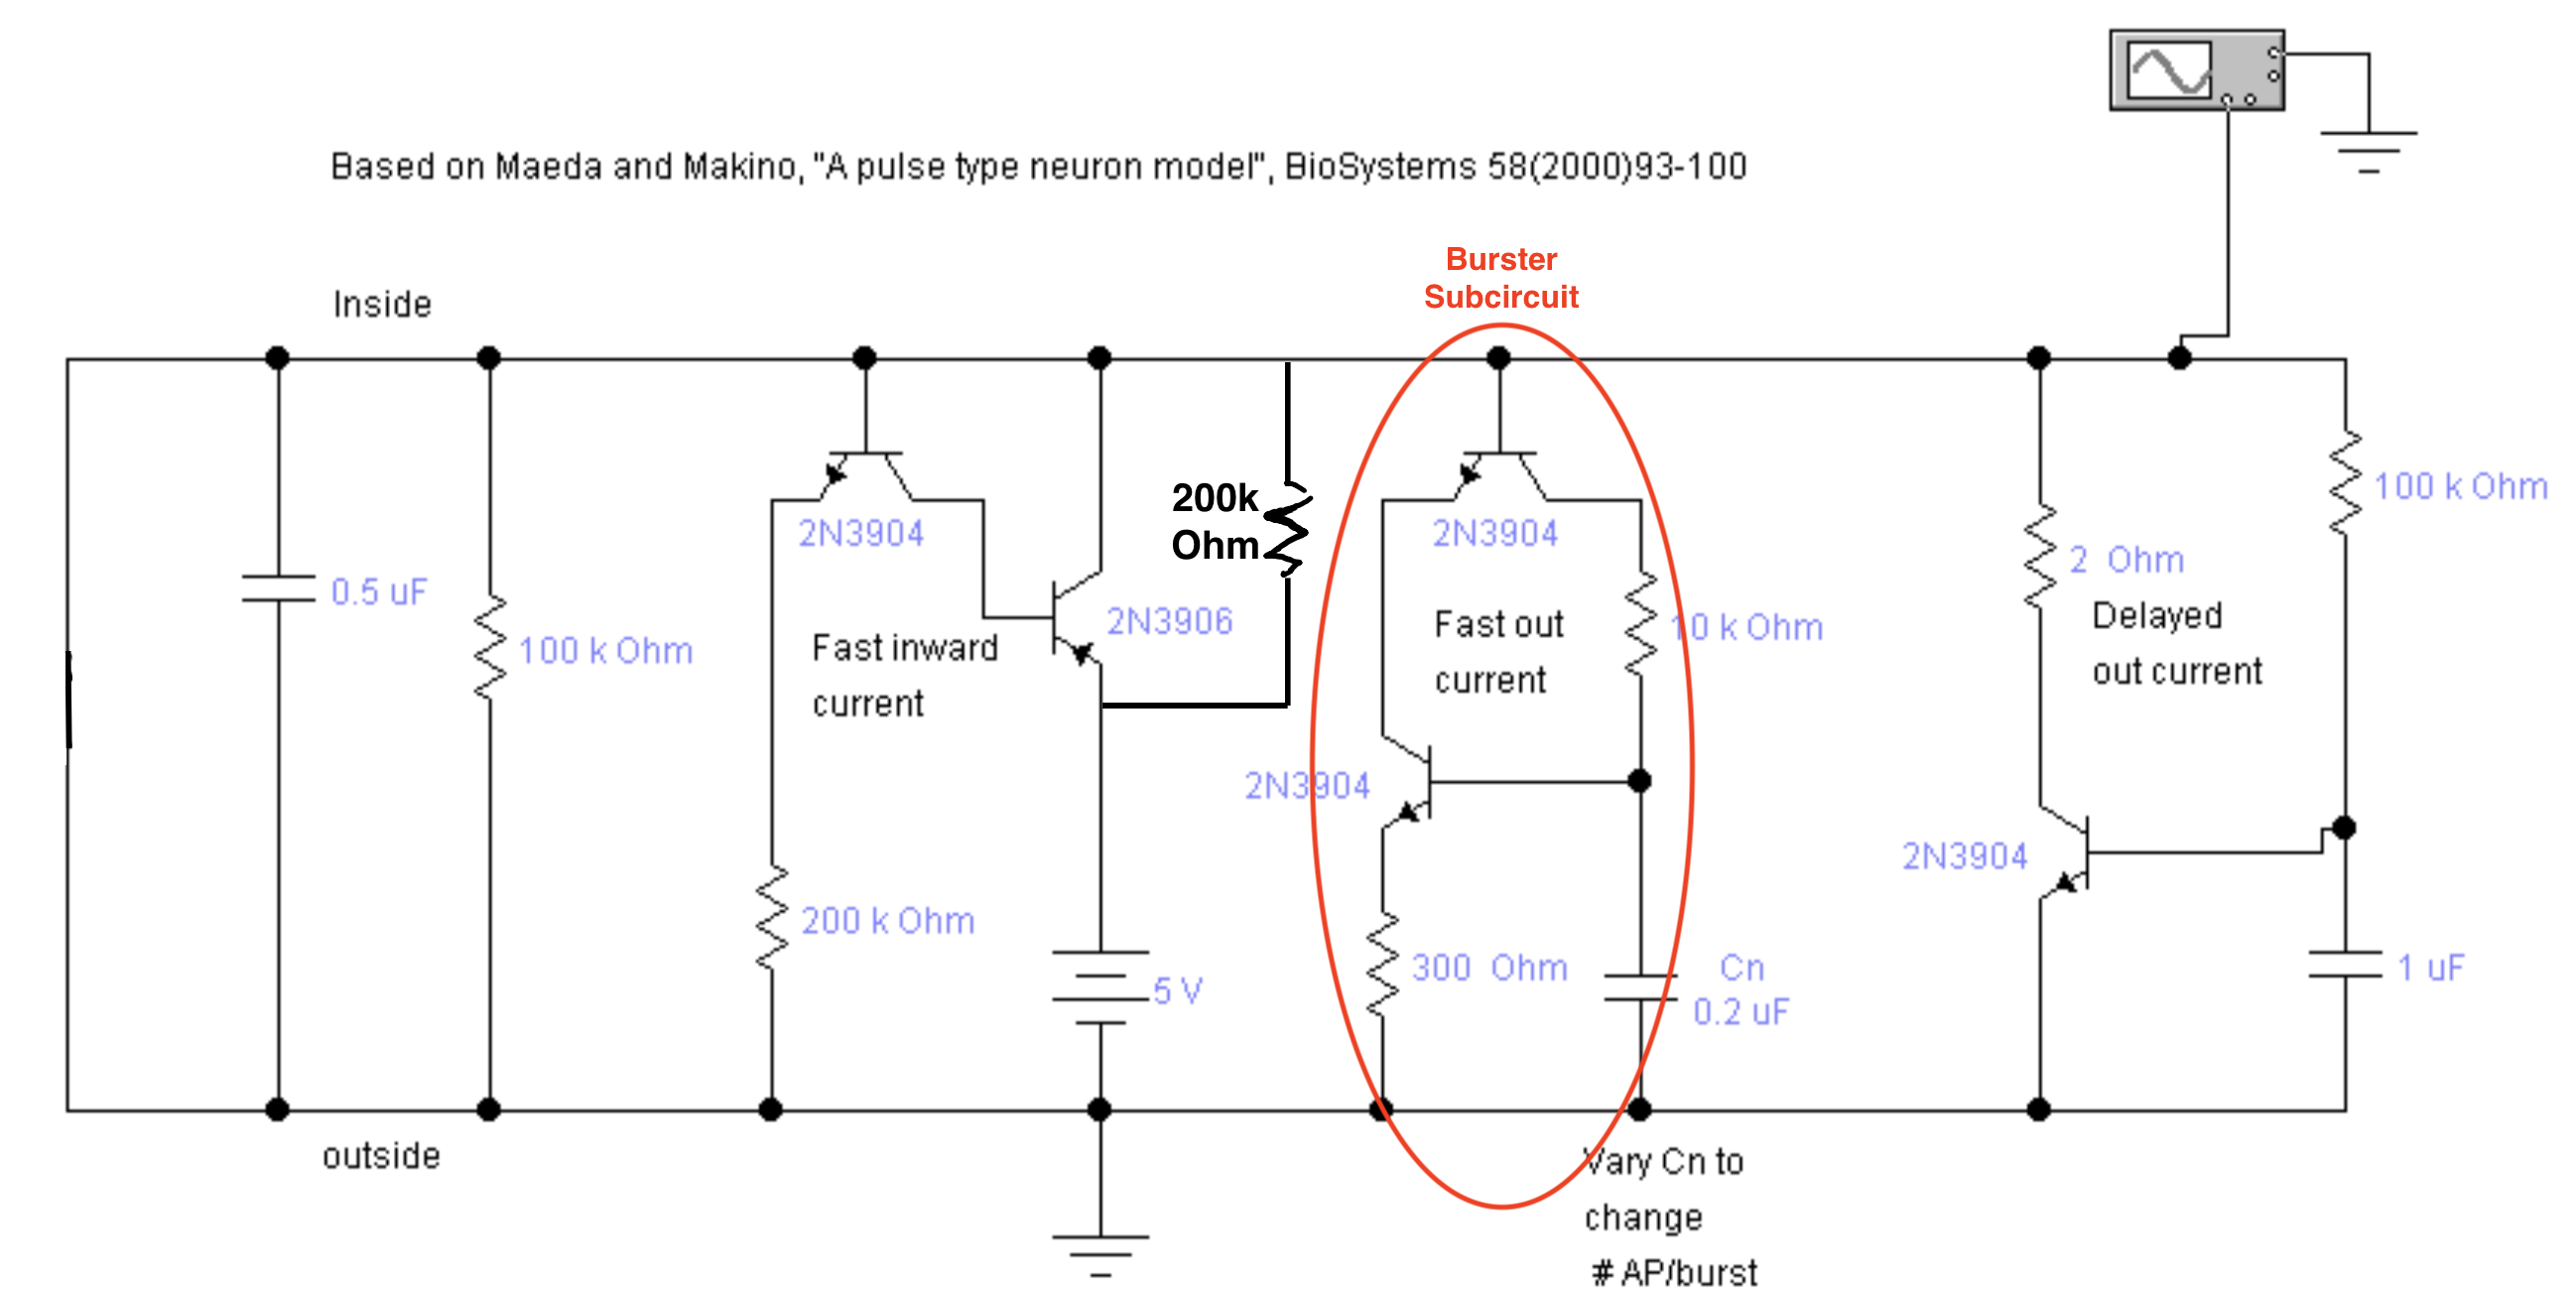
\includegraphics[width=0.7\textwidth]{burster_heart_cell}	
\end{figure}

\begin{figure}[H]
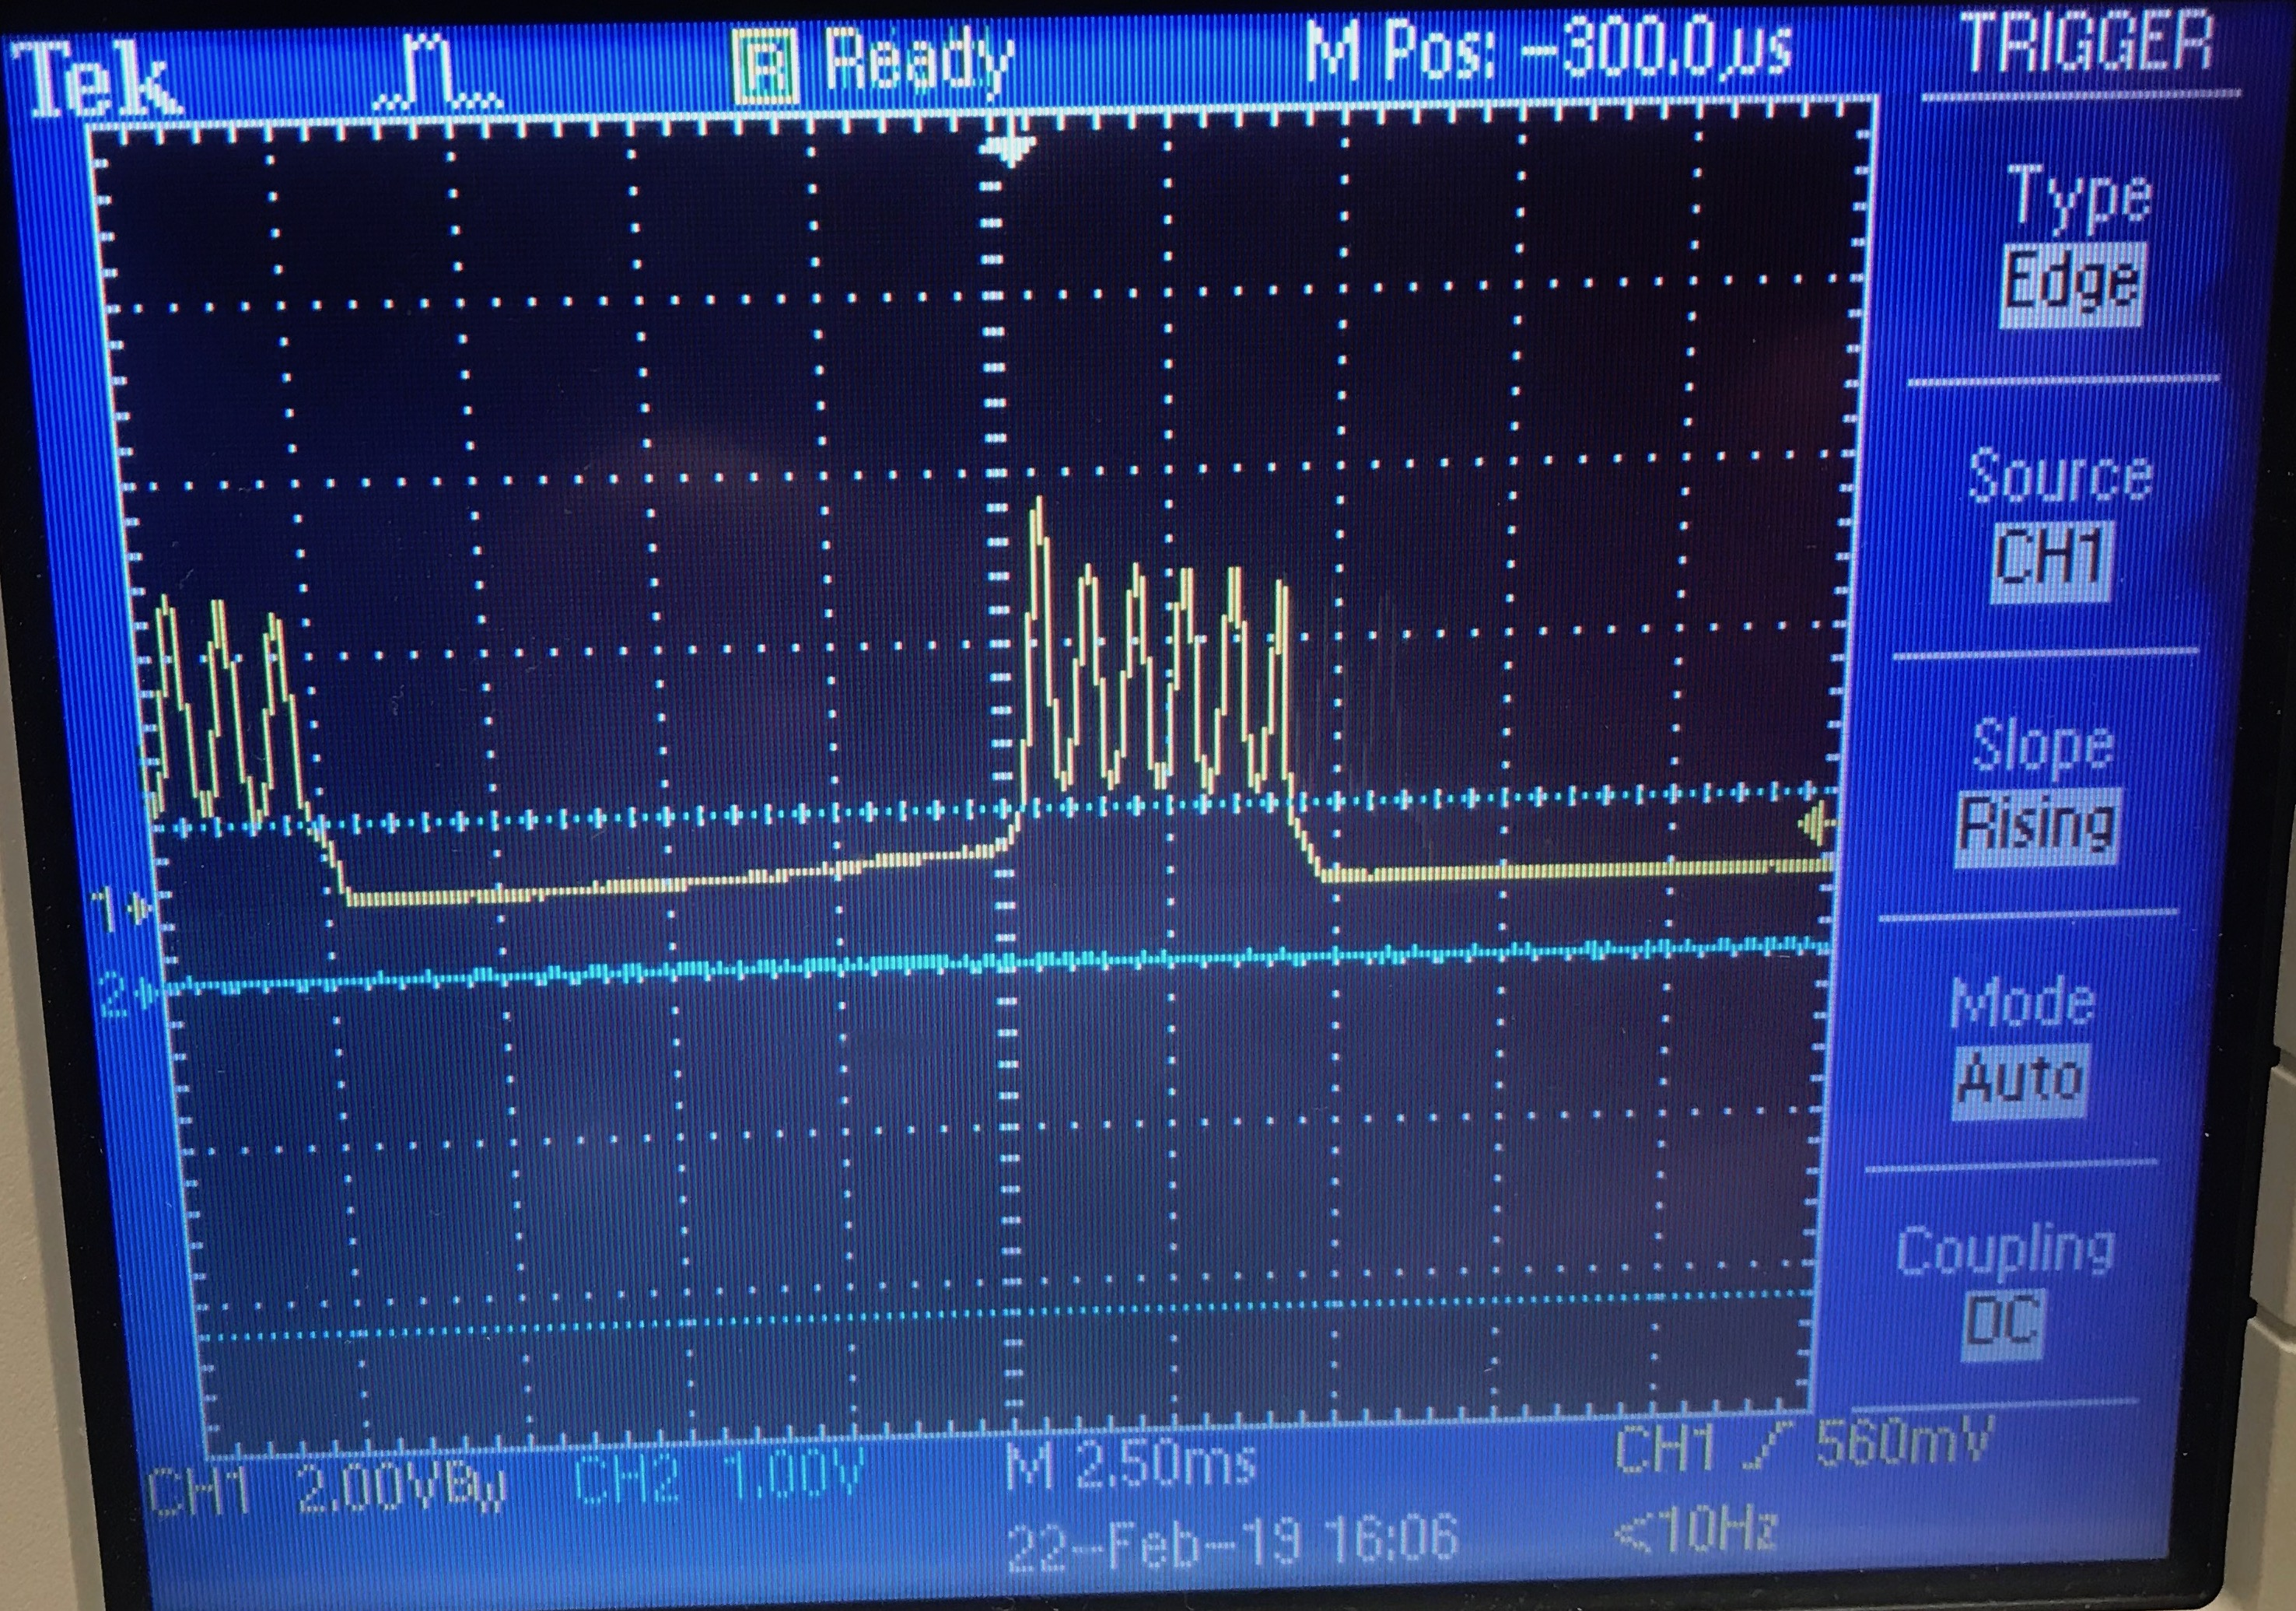
\includegraphics[width=0.5\textwidth]{burster_osc}	
\end{figure}


\bibliography{phy365.bib}
\bibliographystyle{plain}
\nocite{*}


\end{document}
